This work demonstrates the \gls{MSFR} simulation capabilities of Moltres, a
multiphysics simulation tool for \glspl{MSR} \cite{lindsay_introduction_2018}.
To run simulations on Moltres, it requires input
group constant data from a neutron transport solver for the
multigroup neutron diffusion calculations, and a mesh file representing the
geometry of the reactor. This work uses Serpent 2 \cite{leppanen_serpent_2014}
for the former and Trelis \cite{noauthor_trelis_2018} for the latter.
This chapter provides brief introductions of
Serpent 2, MOOSE, and Moltres, and the general modeling approach for the
multiphysics simulations in Moltres.

\section{Serpent 2}

Serpent 2 \cite{leppanen_serpent_2014} is a continuous-energy Monte Carlo
neutron transport application under
active development led by the VTT Technical Research Centre of Finland. It was
created in 2004 for group constant generation in lattice geometries, and has
since grown to support more general capabilities. Serpent 2 is highly
parallelizable, supporting
both MPI and OpenMP parallel programming APIs. It has also been validated and
verified against experimental data and other well-established codes.

In Serpent 2, each neutron is tracked through a combination of
ray-tracing-based surface tracking and rejection sampling-based delta
tracking. Users may define the number of neutron histories and the number of
active and inactive cycles for each
simulation. Inactive cycles are required for fission source distribution
convergence, before interactions are tallied in the active cycles.
Interaction types and locations are
determined stochastically based on neutron interaction data from established
nuclear data libraries (e.g. ENDF \cite{chadwick_endf/b-vii.1_2011}, JEFF
\cite{oecd/nea_jeff-3.1.2_2014}). These nuclear data libraries provide
continuous-energy cross section data at discrete temperatures. Beyond the
discrete library temperatures, Serpent 2 has a built-in Doppler-broadening
preprocessor that extrapolates the relevant cross section data from a lower
temperature \cite{leppanen_serpent_2014}. 

In the context of this work, Serpent 2 uses the JEFF-3.1.2 nuclear
data library \cite{oecd/nea_jeff-3.1.2_2014} to generate group constants
needed by Moltres. The relevant group constant data are collapsed into six
neutron energy groups, and calculated at discrete temperature values from 800
K to 1300 K at 100 K intervals. Table \ref{table:bound} shows the upper bounds
of each neutron energy group. The group constants relevant for neutronics
calculations in Moltres are the
macroscopic fission $\Sigma^f_{g}$, removal $\Sigma^r_{g}$, and scattering
$\Sigma^s_{g' \rightarrow g}$ neutron cross sections,
neutron diffusion coefficients $D_g$, average fission energies $\epsilon_g$,
average neutron yields $\nu$, inverse neutron speeds $1/v$, flux spectra
$\chi$, \gls{DNP} decay constants $\lambda_i$, and effective delayed neutron
fractions $\beta_{eff}$. These group constants are extracted from
the Serpent 2 output files using a Python script available from the Github
repository that holds the Moltres source code \cite{lindsay_moltres_2017}. The
script rewrites the group constants into a Moltres-compatible format.

Serpent 2 provides standard geometric surfaces (e.g. planes, cylinders, cones)
for defining reactor geometries. In this work, the reactor geometry is the
same axisymmetric \gls{MSFR} geometry from the paper by Fiorina et al.
\cite{fiorina_modelling_2014}, as shown in Fig. \ref{fig:msfrgeom}.

\begin{table}[htb!]
	\centering
	\caption{Neutron energy group upper bounds used in Serpent 2.}
	\begin{tabular}{c S}
		\toprule
		{Group number} & {Upper bound [MeV]}\\
		\midrule
		1 & 20\\
		2 & 2.2313\\
		3 & 0.4979\\
		4 & 0.0247875\\
		5 & 0.0055308\\
		6 & 0.0007485\\
		\bottomrule
	\end{tabular}
	\label{table:bound}
\end{table}

\section{MOOSE and Moltres}

Moltres \cite{lindsay_moltres_2017} is a \gls{MOOSE}-based
\cite{gaston_physics-based_2015} application for
coupled neutronics/thermal-hydraulics simulations of \glspl{MSR}. MOOSE
provides foundational framework for computationally solving \glspl{PDE} and
pre-built physics modules for common applications such as the Navier-Stokes
physics module. Moltres is also a MOOSE physics module for simulating
\glspl{MSR}. This section describes MOOSE, the Navier-Stokes physics module,
and Moltres.

\subsection{MOOSE}

\gls{MOOSE} \cite{gaston_physics-based_2015} is a highly parallelizable,
finite element framework developed at \gls{INL} for simplifying the process of
creating fully-coupled, non-linear, multiphysics solvers. The framework
provides a user-friendly interface for this task through object-oriented
programming in C++. All aspects of a typical multiphysics problem, such as the
terms in the \glspl{PDE}, the initial and boundary conditions, the material
properties, etc., are represented in \gls{MOOSE} as C++ objects. New objects
can inherit properties from related old objects to simplify implementation and
reduce code duplication. Overall, this approach
is helpful for many researchers, a significant fraction of whom do not possess
high-level programming backgrounds, as they are unencumbered by the
technical details and complexities involved in programing mesh handling
and \gls{PDE} solving in finite element analysis.

\gls{MOOSE} itself relies heavily on libMesh \cite{kirk_libmesh:_2006} and
PETSc \cite{satish_petsc_2019} for its mesh handling and \gls{PDE} solver
functionalities. As a result, \gls{MOOSE} supports adaptive meshing schemes
and automatic variable scaling amongst other advanced features for improved
accuracy and performance times. Full
coupling is maintained by the execution of Newton-based solves on the
weak formulations of the multiple \glspl{PDE} to minimize the residual values.
Fully-coupled solves are essential for accurately resolving systems with
strongly interacting physics. The \gls{MSR} concept is one such example, where
the neutronics and thermal-hydraulics are tightly coupled through the Doppler
effect and the temperature dependence of liquid fuel salt density.

\gls{MOOSE}, and Moltres by extension, are capable of up to 3-D geometry
modelling. They support a wide range of input mesh file formats listed in a
\gls{MOOSE} webpage, including the commonly used Exodus II file format.
Specifically for the 2-D case, axial symmetry is easily and automatically
imposed by changing one line of code in the input file, without any changes in
the Cartesian representations of the \glspl{PDE} and boundary conditions in
their original C++ implementations. This feature provides significant
computational time savings for 3-D systems that exhibit high axial symmetry.
Another important feature for reducing computational time is the use of MPI
for parallel computing. All \gls{MOOSE}-based codes can be compiled and
run on high performance computing clusters.

\begin{figure}[htb!]
    \centering
    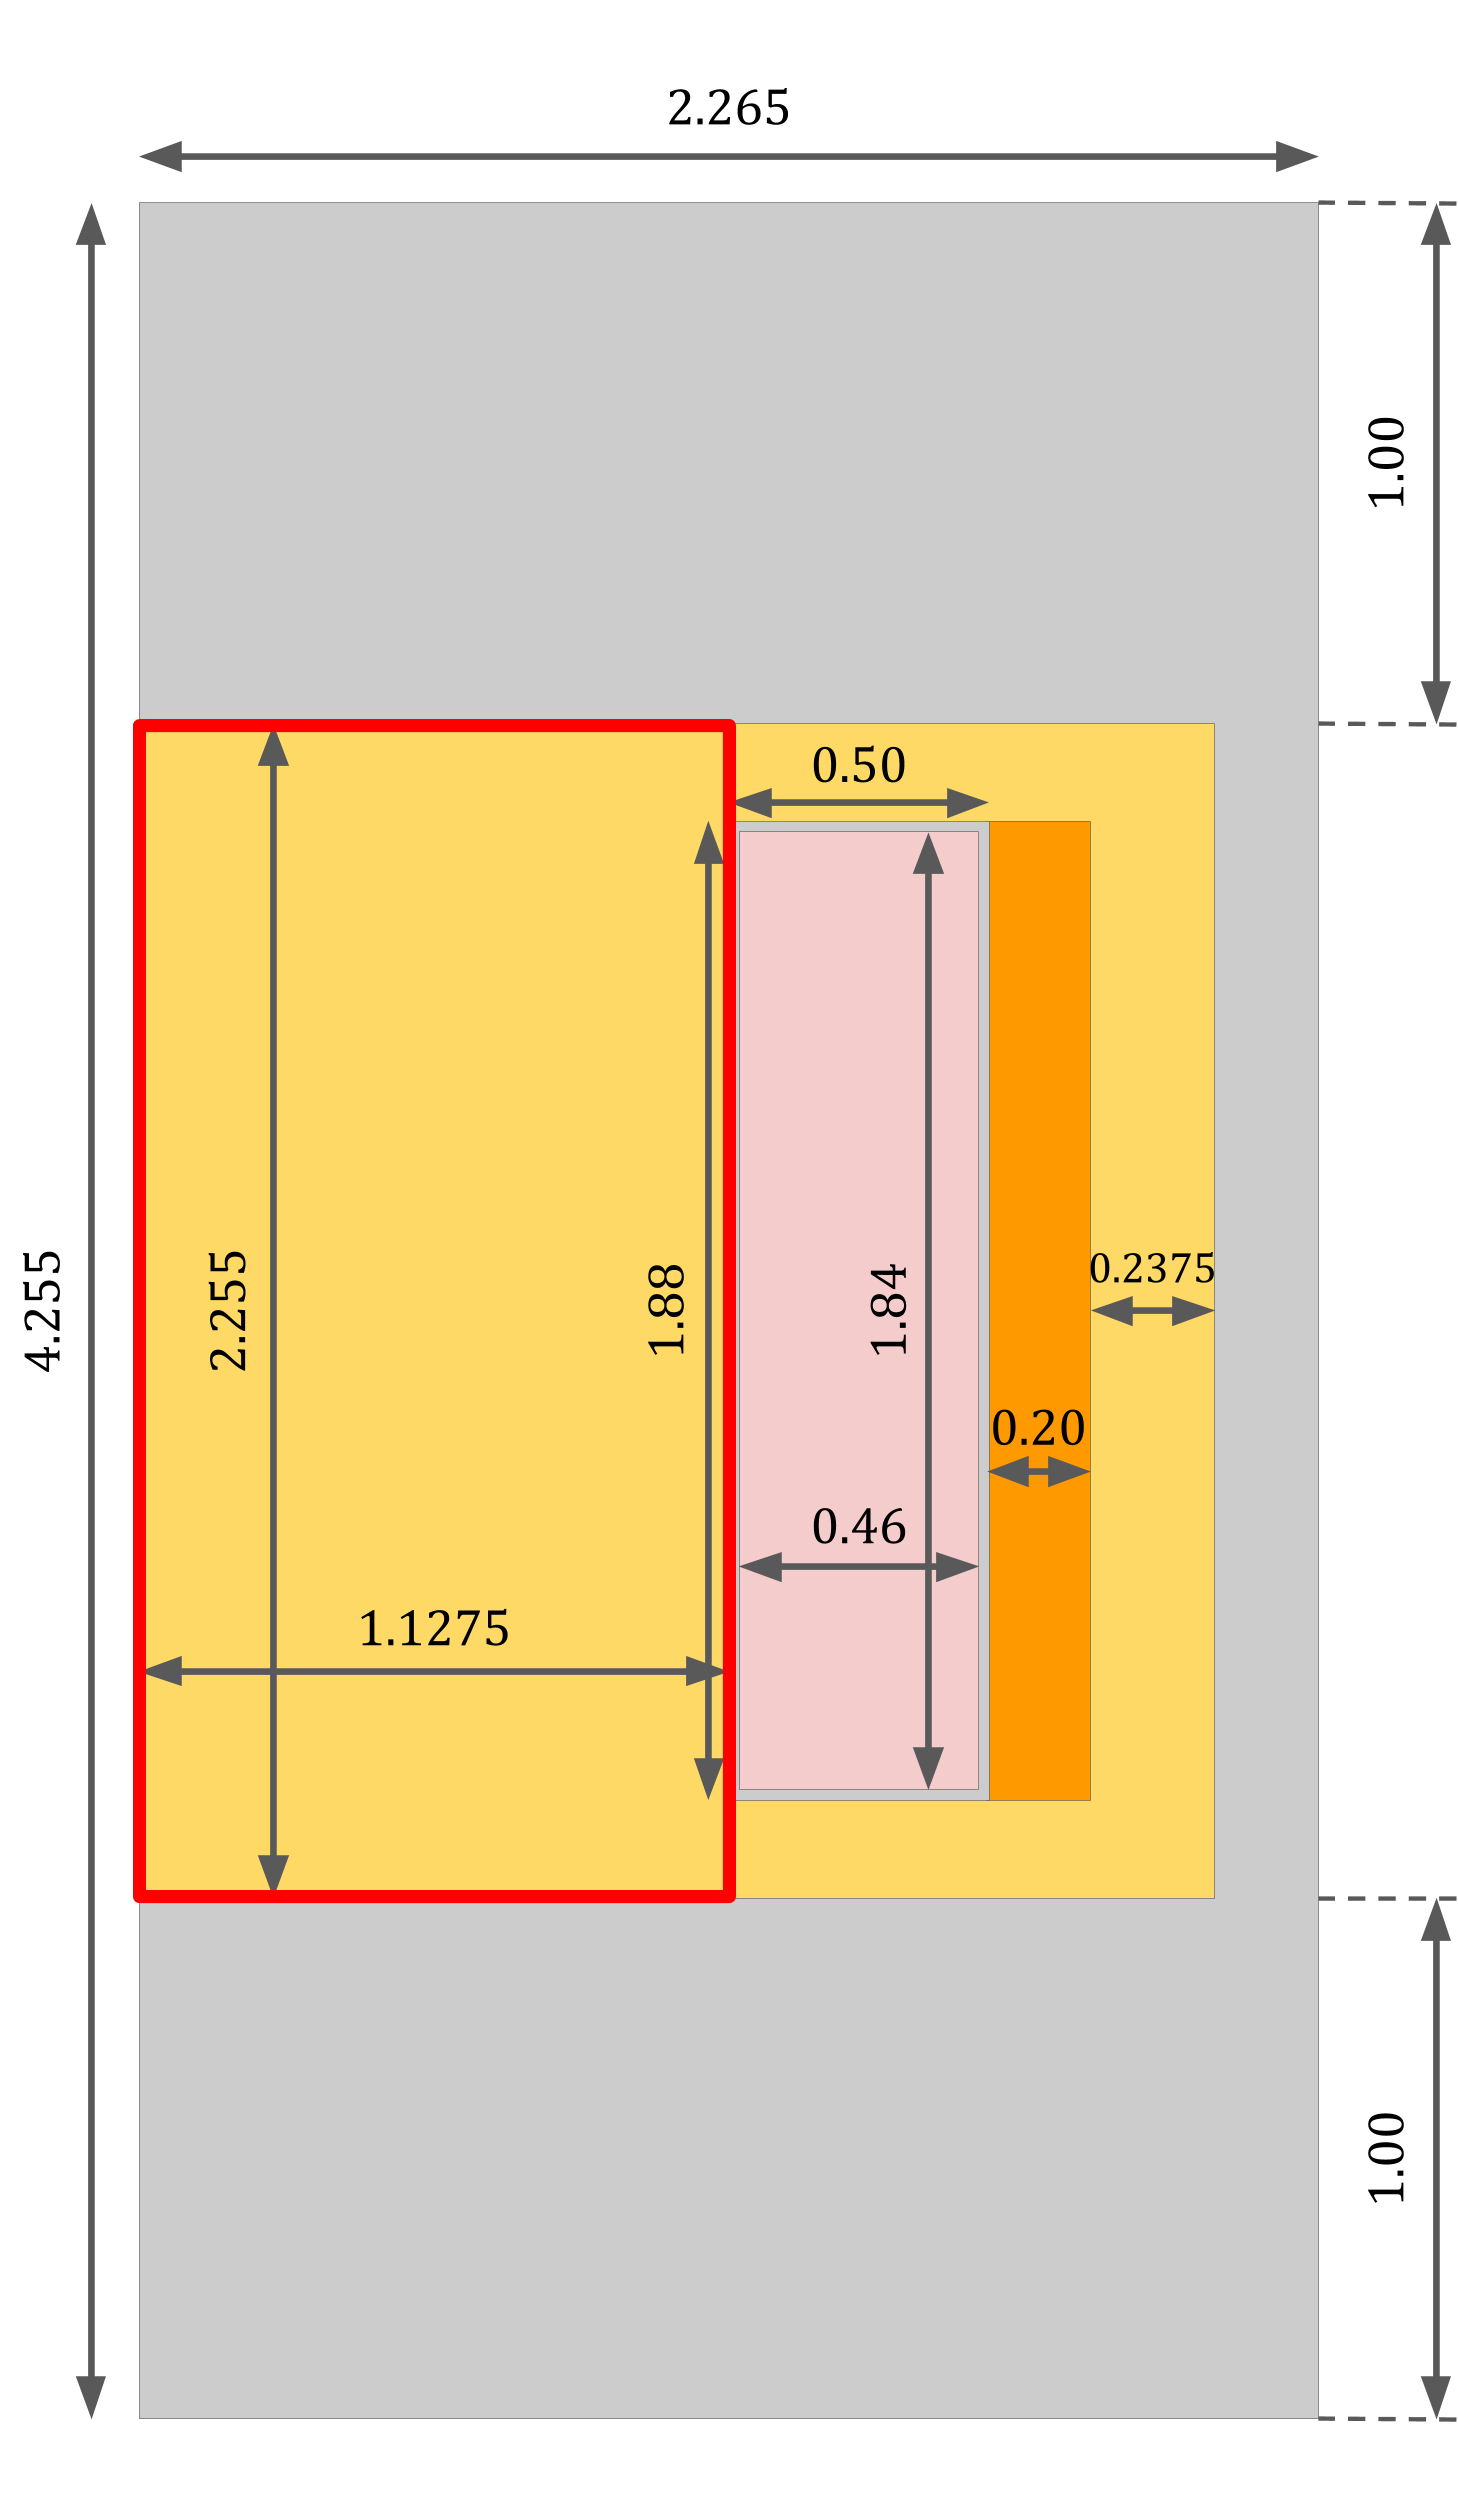
\includegraphics[width=.5\textwidth]{central-core}
    \caption{2-D axisymmetric model of the MSFR. The red box indicates the
    central core region in the modeling approach in Moltres.}
    \label{fig:core}
\end{figure}

As mentioned in the previous chapter, we divided the fuel salt loop into two
regions, the central core region where most of the fissions take place, and
the outer loop region where the heat exchanger is located. The central core
region specifically refers to the central region indicated by
the red box in Figure \ref{fig:core}. We simplified the outer loop
into a 1-D pipe as it is a subcritical region and its main purposes are: to
introduce a out-of-core residence time for the \glspl{DNP}, and to site the
heat exchanger-equivalent object in Moltres.
Accordingly, this section provides separate descriptions for the governing
equations in the central core region and the outer loop region. There is also
a third region comprising of the blanket salt, the Ni-alloy reflectors, 
and other material . This region is important for capturing an accurate
estimate of neutron leakage as opposed to simpler approximations such as
imposing fixed albedo boundary conditions on the neutron fluxes.

\subsection{Central Core Region}

The central core region is of greatest interest to us during steady state and
transient scenarios; the center of the reactor is naturally where most of the
fissions and heat generation occur. Consequently, the \glspl{PDE} solved for
in this region are in their most complete form relatively to simplifying
assumptions found in the other regions.

\subsubsection{Neutronics Model}

The neutron flux calculations in the central core region are
performed using the standard formulations for the time-dependent multigroup
neutron diffusion equations and \gls{DNP} concentration equations as shown in
equations \ref{eq:neut} and \ref{eq:dnp}:
%
\begin{align}
    \frac{1}{v_g} \frac{\partial \phi_g}{\partial t} &= \nabla \cdot D_g
    \nabla \phi_g - \Sigma^r_g \phi_g +
    \sum^G_{g' \neq g} \Sigma^s_{g' \rightarrow g} \phi_{g'} + \chi^p_g
    \sum^G_{g'=1} (1-\beta) \nu \Sigma^f_{g'} \phi_{g'} + \chi^d_g \sum^I_i
    \lambda_i C_i, \label{eq:neut} \\
    \frac{\partial C_i}{\partial t} &= \beta_i \sum^G_{g'=1} \nu \Sigma^f_{g'}
    \phi_{g'} - \lambda_i C_i - \boldsymbol{u} \cdot \nabla C_i + \nabla \cdot
    D_t \nabla C_i, \label{eq:dnp} \\
    \intertext{where}
    v_g &= \text{average speed of neutrons in group $g$ [cm s$^{-1}$],} 
    \nonumber \\
    \phi_g &= \text{neutron flux in group $g$ [cm$^{-2}$ s$^{-1}$],} \nonumber
    \\
    t &= \text{time [s],} \nonumber \\
    D_g &= \text{diffusion coefficient of neutrons in group $g$ [cm$^2$
    s$^{-1}$],} \nonumber \\
    \Sigma^r_g &= \text{macroscopic cross section for removal of neutrons from
    group $g$ [cm$^{-1}$],} \nonumber \\
    \Sigma^s_{g' \rightarrow g} &= \text{macroscopic cross section of
    scattering from $g'$ to $g$ [cm$^{-1}$],} \nonumber \\
    \chi^p_g &= \text{prompt fission spectrum for neutrons in group $g$,}
    \nonumber \\
    G &= \text{total number of discrete neutron groups,} \nonumber \\
    \nu &= \text{average number of neutrons produced per fission,} \nonumber
    \\
    \Sigma^f_{g} &= \text{macroscopic fission cross section for neutron in
    group $g$ [cm$^{-1}$],} \nonumber \\
    \chi^d_g &= \text{delayed fission spectrum for neutrons in group $g$,}
    \nonumber \\
    I &= \text{total number of delayed neutron precursor groups,} \nonumber \\
    \beta &= \text{total delayed neutron fraction,} \nonumber \\
    \beta_i &= \text{delayed neutron fraction of precursor group $i$,}
    \nonumber \\
    \lambda_i &= \text{average decay constant of delayed neutron precursors in
    precursor group $i$ [s$^{-1}$],} \nonumber \\
    C_i &= \text{concentration of delayed neutron precursors in precursor
    group $i$ [cm$^{-3}$],} \nonumber \\
    D_t &= \text{turbulent diffusion of the delayed neutron precursors [cm$^2$
    s$^{-1}$].} \nonumber
\end{align}
%

While the limitations of the multigroup neutron diffusion compared to other
deterministic and Monte Carlo methods, particularly for flux values near
boundaries, are well-documented, the diffusion model provides acceptable
accuracy at lower computational costs. Moreover, the central core region
contains no material interfaces except at its boundaries. The Neutronics
results section provides a comparison of the \gls{MSFR} multiplication factor
values and reactivity coefficients between Moltres and Serpent.

The \gls{DNP} concentration equation has additional advection and turbulent
diffusion terms to account for the movement of \glspl{DNP} in the primary
coolant loop. The turbulent diffusion value is governed by the following
equation:
%
\begin{align}
    D_t &= \frac{\mu_t}{\rho Sc_t}
    \intertext{where}
    \mu_t &= \text{ eddy viscosity [Pa s],} \nonumber \\ 
    \rho &= \text{ density of the fuel salt [kg m$^{-3}$],} \nonumber \\
    Sc_t &= \text{ turbulent Schmidt number.} \nonumber
\end{align}
%

We assumed $Sc_t = 0.85$ for a fair comparison with the Polimi/TUDelft
models which used the same value.

\begin{figure}[htb!]
    \centering
    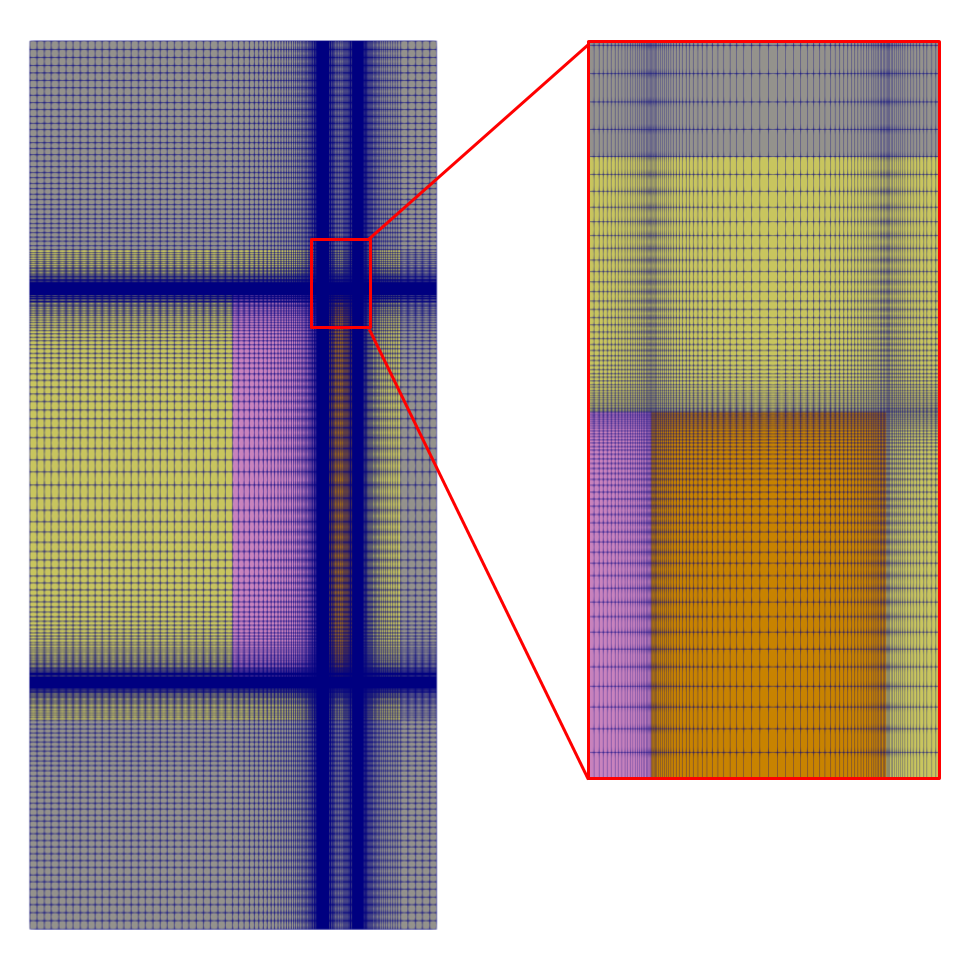
\includegraphics[width=.8\textwidth]{mesh}
    \caption{Mesh adopted in Moltres and a close-up view of the mesh around
    the boron carbide absorber.}
    \label{fig:mesh}
\end{figure}

Moltres users may vary the total number of neutron energy groups as
long as they provide Moltres with the appropriate group constant data. The
number of precursor groups is also variable, though usually predetermined by
the choice of nuclear data library in the group constant generation step.
Moltres automatically interpolates the group constant data for required
temperatures using one of the many predefined interpolation methods available
in \gls{MOOSE}. Once again, users have the freedom to select their
interpolation method of choice.

For this work, we have six neutron energy groups according to the energy
boundaries in table \ref{table:bound}, eight \gls{DNP} groups as defined by
the JEFF-3.1.2 library, and the spline interpolation method. The neutron flux
and \gls{DNP} concentration values were approximated by first-order Lagrange
and constant monomial shape functions respectively on the finite element mesh.
Figure \ref{fig:mesh} shows the mesh adopted for the \gls{MSFR} model.
We assumed vacuum boundary conditions for all six neutron group fluxes along
the external boundaries of the geometry, and homogeneous Neumann boundary
conditions along the axial symmetry boundary. For the \gls{DNP}
concentrations, we imposed homogeneous Neumann boundary conditions on the
walls, and inflow and outflow boundary conditions on the inlet and outlet
boundaries respectively. The inlet \gls{DNP} concentration values were
imported from the outlet values of the 1-D outer loop pipe at the same
timestep.

For the decay heat model, a previous study on the MSFR by Aufiero et al.
\cite{aufiero_extended_2013} had shown that using three decay heat precursor
groups with different half-lives in the form of exponential equations, can
accurately model decay heat in the MSFR for up to 300 seconds after shutdown
with a relative error of less than 2\%. Thus, we implemented a decay heat
model using the following equation:
%
\begin{align}
	\frac{\partial \omega_k}{\partial t} &= f_k \sum^G_{g=1} \epsilon_{g}
	\Sigma^f_{g} \phi_{g} - \lambda^k \omega_k - \boldsymbol{u} \cdot \nabla
	\omega_k + \nabla \cdot D_t \nabla \omega_k, \label{eq:decayheat} \\
	\intertext{where}
    \omega_k &= \text{total decay heat power density from decay heat
    precursors in group $k$ [W cm$^{-3}$]} \nonumber \\
	f_k &= \text{fraction of decay heat to total power at steady state}
	\nonumber \\
	\epsilon_g &= \text{average fission energy per fission [W]} \nonumber \\
	\lambda^k &= \text{average decay constant of decay heat precursors in
	group $k$ [s$^{-1}$].} \nonumber
\end{align}

Like the neutron and \gls{DNP} groups, Moltres can take an arbitrary number of
decay heat groups. In this work, as with the other parameters, we used the
same decay heat fractions and decay constants, shown in Table
\ref{eq:decayheat}, used in the Polimi/TUDelft models for three decay heat
groups.

\begin{table}[htb!]
	\centering
	\caption{Decay heat group parameters \cite{fiorina_modelling_2014}.
	$\lambda_i$ and $f_i$ are the decay constants and decay heat fractions
	associated to group $i$.}
	\begin{tabular}{S S S}
		\toprule
		{Decay heat group} & {$\lambda_i$ [s$^{-1}$]} & {$f_i$} \\
		\midrule
		1 & 0.1974 & 0.0117 \\
		2 & 0.0168 & 0.0129 \\
		3 & 0.000358 & 0.0186 \\
		\bottomrule
	\end{tabular}
	\label{table:decayheat}
\end{table}

\subsubsection{Thermal-Hydraulics Model}

Fluid dynamics in Moltres can be modeled using the \gls{INS} equations with
the Boussinesq hypothesis for eddy viscosity. Most of the Navier-Stokes
capabilities in Moltres is derived from the MOOSE Navier-Stokes module
\cite{peterson_overview_2017}. The standard \gls{INS} equations are:
%
\begin{align}
    \text{Momentum eq.:} && \rho \frac{\partial \boldsymbol{u}}{\partial t} &=
    -\rho (\boldsymbol{u}
    \cdot \nabla) \boldsymbol{u} + \nabla \cdot (-p \boldsymbol{I} + \mu [
    \nabla \boldsymbol{u} + (\nabla \boldsymbol{u})^T] + \boldsymbol{f} &&
    \label{eq:momemtum} \\
    \text{Divergence-free:} && \nabla \cdot \boldsymbol{u} &= 0 &&
    \label{eq:divergence}
    \intertext{where}
    && p &= \text{ pressure [Pa],} && \nonumber \\
    && \mu &= \text{ dynamic viscosity [Pa s],} && \nonumber \\
    && \boldsymbol{f} &= \text{ body force per unit volume [N m$^{-3}$].} &&
    \nonumber
\end{align}

In addition to the intrinsic molecular viscosity, we introduced an eddy
viscosity term to approximate turbulent flow effects. The current
implementation of Moltres does not have a turbulence model such as the
\gls{RANS} models used in the Polimi/TUDelft models. Thus, we made a
zeroth-order approximation of the eddy viscosity based on the results reported
in the Polimi/TUDelft models. The eddy viscosity is assumed to be 40 Pa s.
Despite the simplicity of this assumption, we were able to reproduce much of
the flow profile observed in the Polimi/TUDelft models at steady state.

The energy balance equation for temperature is
given in Eq. \ref{eq:temp}. The diffusion term includes turbulent heat
diffusivity based on the eddy viscosity $\mu_t$ and the turbulent Prandtl
number $Pr_t$, which we assume to be equal to 0.85. 
%
\begin{align}
    \rho c_{p} \frac{\partial T}{\partial t} &= - \rho c_p \boldsymbol{u}
    \cdot \nabla T + \nabla \cdot [(k + k_t) \nabla T] + Q_s
    \label{eq:temp} \\
    k_t &= \frac{\mu_t}{\rho Pr_t} \\
    Q_s &= \Big( 1 - \sum^K_{k=1} f_k \Big) \sum^G_{g=1} \epsilon_g \Sigma_g^f
    \phi_g + \sum^K_{k=1} \omega_k, \label{eq:source}
    \intertext{where}
    c_p &= \text{specific heat capacity of molten salt [J kg$^{-1}$ K$^{-1}$],
    } \nonumber \\
    T &= \text{temperature of molten salt [K]} \nonumber \\
    \boldsymbol{u} &= \text{velocity of molten salt [m s$^{-1}$],} \nonumber
    \\
    k &= \text{thermal conductivity of molten salt [W m$^{-1}$ K$^{-1}$],}
    \nonumber \\
    K &= \text{total number of decay heat groups.} \nonumber
\end{align}
%
The first term in the heat source $Q_s$ represents prompt fission heat, and
the second term represents decay heat from the $K$ decay heat groups.

We expect good qualitative agreement with the Polimi/TUDelft models,
including the large recirculation region near the blanket tank walls and the
resulting high temperatures in that region. There would be some minor
discrepancies where the viscosity values are under- or over-predicted, leading
to slightly inaccurate temperature and precursor concentration values from
turbulent diffusion.

\subsection{Outer Loop Region}

Moltres also accounts for the decay of
\glspl{DNP} outside the central core region by simulating its flow in a
separate 1-D pipe geometry. This outer loop pipe simulation is implicitly
coupled to the active core simulation through Picard iterations in MOOSE's
MultiApp functionality and inlet/outlet boundary values. For this work with
the \gls{MSFR} model, we assumed a pipe
length of 2.255 m with salt flowing at 1.1275 m s$^{-1}$ for an average
out-of-core residence time of 2 seconds to follow the design specifications.

\subsubsection{Neutronics Model}

Since this region is largely subcritical, the only significant
neutronics-related phenomena are the drift, and decay of \glspl{DNP}.
The governing equation for the \glspl{DNP} is:
%
\begin{align}
    \frac{\partial C_i}{\partial t} &= - \lambda_i C_i - u
    \frac{\partial C_i}{\partial x} + D_t \frac{\partial^2 C_i}{\partial x^2}.
    \label{eq:dnploop}
\end{align}
%
Equation \ref{eq:dnploop} is derived from equation \ref{eq:dnp} by removing
the fission \gls{DNP} source term, and the conversion of the advection and
diffusion terms to their 1-D forms. The decay constants and diffusion
coefficient are the same values used in the central core region.

\subsubsection{Thermal-Hydraulics Model}

Instead of the Navier-Stokes equations, we have a predetermined velocity of
1.1275 m s$^{-1}$ in the outer loop region. The governing equation for
temperature, derived from equation \ref{eq:temp}, is:
%
\begin{align}
    \rho c_{p} \frac{\partial T}{\partial t} &= - \rho c_p u
    \frac{\partial T}{\partial x} - Q_{hx} \label{eq:temploop} \\
    Q_{hx} &= \alpha (T - T_i) \delta (x_0) \label{eq:hx} \\
    \intertext{where}
    \alpha &= \text{heat transfer coefficient [W K$^{-1}$],} \nonumber \\
    x_0 &= \text{position of the point heat exchanger [m].} \nonumber
\end{align}

The fission heat source term is replaced with a heat exchanger sink term
which depends on the temperature difference between the fuel salt $T$ and the
secondary loop salt $T_s$. For simplicity, we assumed a constant temperature
of 823 K in the secondary loop. The heat transfer coefficient was determined
by assuming that the fuel outlet temperature is 1023 K and calculating the
heat removal rate to induce a 100 K drop at the given volumetric flow rate
and heat capacity of the fuel salt. We opted to ignore the diffusion term due
to the discontinuity of the temperature distribution across the point heat
exchanger. 

\subsection{Boundary Conditions and Flow Transfers}

This subsection details the various boundary conditions for all of the
tracked variables, and the \gls{DNP} and temperature flow transfers between
the central core and outer loop regions. 

Starting with the central core region, for the neutron group fluxes, we
imposed vacuum boundary conditions on the
outermost boundaries of the geometry in Figure \ref{fig:core} excluding the
axial boundary. The \gls{DNP} variables have homogeneous Neumann boundary
conditions along the axis and the walls in the central core region, and inflow
and outflow boundary conditions on the inlet and outlet boundaries,
respectively. The temperature variable shares the same type of boundary
conditions as the \gls{DNP} variables.

The flow rate is dictated by an inflow boundary condition at the core inlet
for a volumetric flow rate of 4.5 m$^3$ s$^{-1}$. We imposed no-slip boundary
conditions on the walls of the central core, and homogeneous Neumann boundary
conditions on the outlet. Along the axial boundary, we have homogeneous
Dirichlet boundary condition for the radial velocity component, and
homogeneous Neumann boundary condition for the axial velocity component.

At every timestep, Moltres also calculates weighted averages of the
temperature and \gls{DNP} at the outlet. These values are weighted by the
outflow velocity values at the outlet according to the following equation:
%
\begin{align}
    \overline{\phi} &= \frac{\int_\mathcal{C} \phi(y) u(y) dy}{
    \int_\mathcal{C} u(y) dy} \\
    \intertext{where}
    \phi &= \text{variable to be weighted} \nonumber \\
    \mathcal{C} &= \text{outlet boundary curve} \nonumber \\
    u &= \text{outflow velocity perpendicular to the outlet boundary [m
    s$^{-1}$].} \nonumber
\end{align}

This outflow value from the central core region is transferred to the 1-D
outer loop region as input for the inhomogeneous Dirichlet boundary
condition at the inlet boundary. Likewise, the outflow value from the outer
loop region is used for the inflow value in the central core region. No
averaging is required for this step as the outer loop region is a 1-D system.
We assume that the inflow temperature and \gls{DNP} are uniform at the inlet.
The Picard iterations within every timestep ensure that the two systems are
implicitly coupled even though they're solved separately.
